\section{Justificación}

% ayudaria, contribuiria utilizar este tipo de verbos copreterito

% la primera oración sigue en pareciendo problema.
Debido a la creciente demanda de alimentos \cite{wik_pingali_brocai_2008}, es imperativo que los agricultores de Samalayuca, Chihuahua, cuenten con herramientas de bajo costo que les permitan tomar decisiones basadas en información. El monitoreo constante de los parámetros que tienen mayor influencia sobre el cultivo les ayudará a identificar situaciones que puedan fomentar la aparición de enfermedades. Asimismo, la automatización de tareas que demandan constancia y precisión, como lo son el riego y el control del clima, contribuirá a la estabilización de estos parámetros, disminuyendo el estrés provocado en las plantas. Esto permitirá que los agricultores locales puedan competir contra extranjeros que producen en ambientes controlados y automatizados. 

Esta solución tendrá un impacto económico ya que podrá ser fácilmente replicada en otros invernaderos donde exista un clima similar. Para regiones con climas distintos, se podrán adaptar las reglas de control para las necesidades particulares de la región. Asimismo, este sistema continuará siendo atractivo para quienes busquen una solución de bajo costo. En la Figura \ref{fig:costo_estimado} se puede observar el costo estimado que tendrán los componentes del proyecto.


\begin{figure}[!ht]
    \centering
    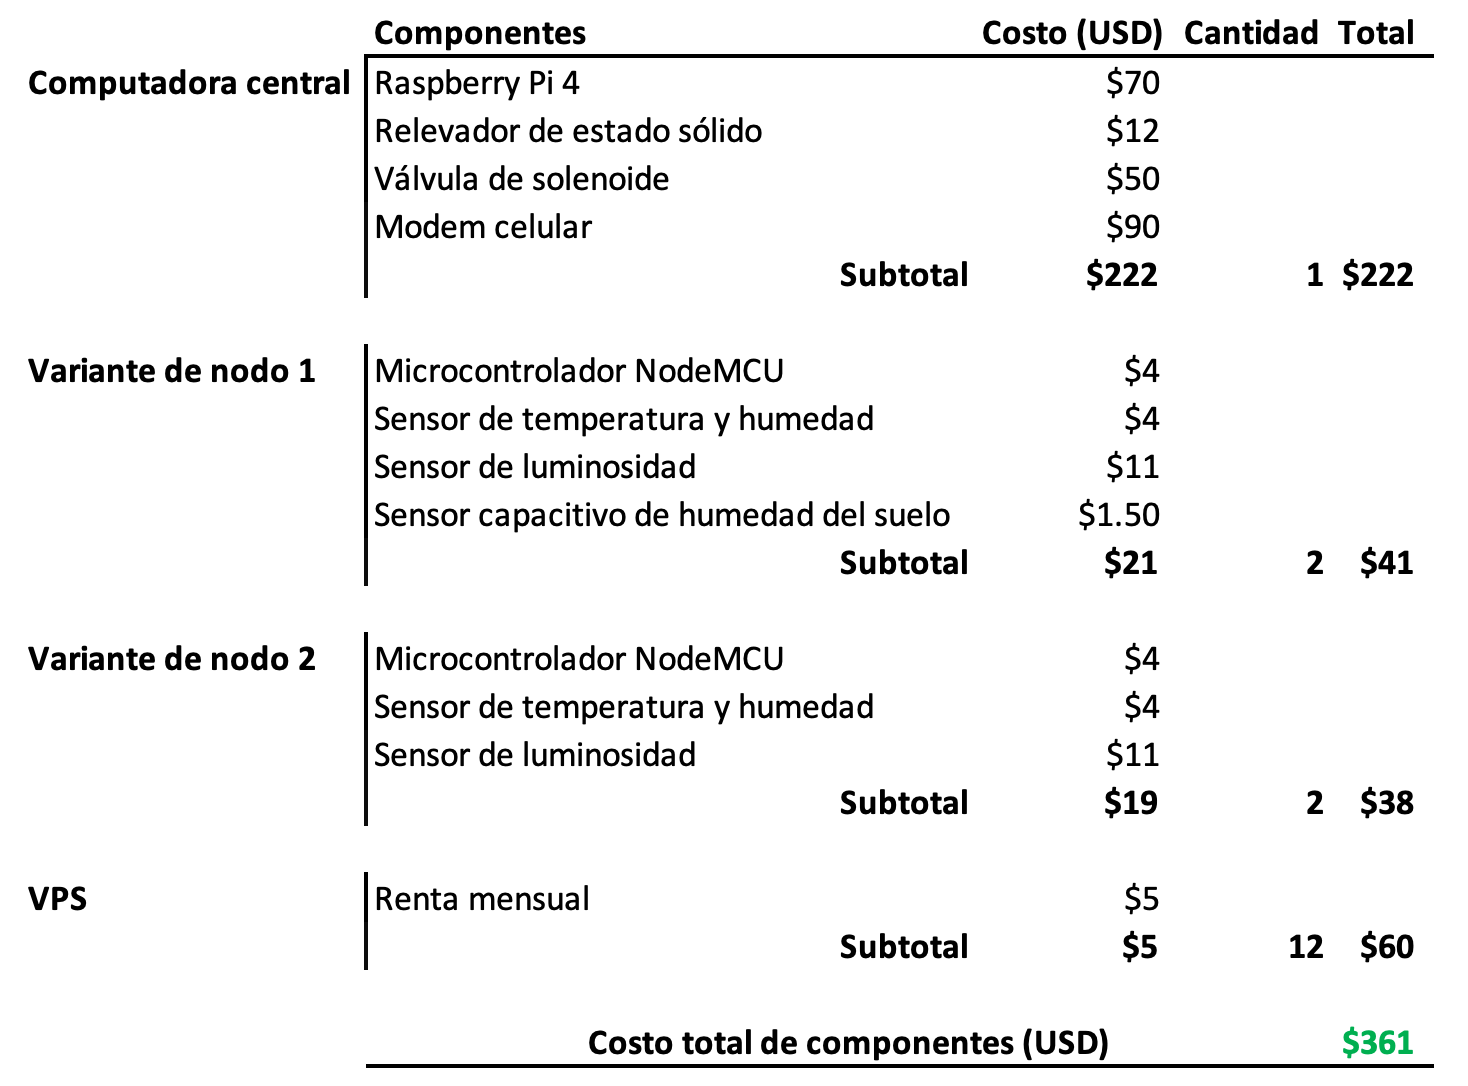
\includegraphics[width=1\linewidth]{imagenes/costo_estimado_proyecto.png}
    \caption{Costo estimado del proyecto }
    \label{fig:costo_estimado}
\end{figure}



